\documentclass[11pt,a4paper]{article}
\usepackage[T1]{fontenc}
\usepackage[utf8]{inputenc}
\usepackage[english]{babel}
\usepackage{lmodern}
\usepackage[a4paper,margin=2.8cm,top=2.6cm,bottom=3cm]{geometry}
\usepackage{amsmath,amssymb,amsthm,mathtools}
\usepackage{booktabs,array}
\usepackage[shortlabels]{enumitem}
\usepackage{microtype}
\usepackage{setspace}
\usepackage[parfill]{parskip}
\usepackage{xcolor}
\usepackage{tikz}
\usetikzlibrary{arrows.meta,positioning,calc}
\usepackage[most]{tcolorbox}
\usepackage[font=small,labelfont=bf,skip=6pt]{caption}
\usepackage[hidelinks]{hyperref}

\setstretch{1.12}
\widowpenalty=10000
\clubpenalty=10000
\setlist{itemsep=3pt,topsep=4pt}
\setlength{\parskip}{0.65\baselineskip}

\definecolor{sininen}{HTML}{0054E9}
\newtcolorbox{intuitio}{enhanced,breakable,colback=sininen!3,colframe=sininen!45,boxrule=0.4pt,
  leftrule=2.5pt,arc=1pt,left=9pt,right=9pt,top=5pt,bottom=5pt,
  title={Intuition},fonttitle=\small\bfseries,coltitle=sininen!80!black,
  attach title to upper={\quad},before skip=8pt,after skip=10pt}

\theoremstyle{plain}
\newtheorem{lause}{Theorem}
\newtheorem{lemma}{Lemma}
\newtheorem{propositio}{Proposition}
\newtheorem{seuraus}{Corollary}
\theoremstyle{definition}
\newtheorem{maaritelma}{Definition}
\newtheorem{oletus}{Assumption}
\theoremstyle{remark}
\newtheorem{huomautus}{Remark}

\newcommand{\E}{\mathbb{E}}
\renewcommand{\P}{\mathbb{P}}
\newcommand{\cC}{\mathcal{C}}
\newcommand{\cZ}{\mathcal{Z}}
\newcommand{\cT}{\mathcal{T}}
\newcommand{\cF}{\mathcal{F}}
\newcommand{\cB}{\mathcal{B}}
\newcommand{\cG}{\mathcal{G}}
\newcommand{\cH}{\mathcal{H}}
\newcommand{\cA}{\mathcal{A}}
\newcommand{\1}{\mathbf{1}}
\newcommand{\pol}[1]{\texttt{#1}}
\newcommand{\Bin}{\operatorname{Bin}}
\newcommand{\Poi}{\operatorname{Poisson}}
\newcommand{\Beta}{\operatorname{Beta}}
\DeclareMathOperator*{\argmax}{arg\,max}
% Table rows from a file; the primitive \input works inside a tabular environment.
\newcommand{\rivit}[1]{\csname @@input\endcsname #1 }

\title{\textbf{The Value of Targeting Gritting\\ with Phone Vibration Detections}\\[6pt]
\large The mathematical model of the slipperiness simulator, with proofs}
\author{Elias Wuolijoki\\[2pt] \small Junction Turku 2026, If challenge}
\date{18 October 2026}

\begin{document}
\maketitle

\begin{abstract}
\noindent
We study a simulator in which pedestrians' phones detect slips from vibration and
gritting is directed by these detections. The walkable squares of central Turku
have a hidden slipperiness that changes daily and that nobody observes directly.
The maintenance crew can grit only a few blocks at a time, and a block may not be
gritted again before the effect of its previous gritting has ended.

We prove that targeting based on the beta-binomial posterior computed from the
detections yields, in expectation, at most as many falls as any policy that
ignores the detections. Compared with the best such policy, the improvement is
strictly positive exactly when slipperiness varies between squares and the
detector distinguishes slips from false alarms. The results concern the simulated
world, not real streets in Turku or If's claims.
\end{abstract}

\vspace{4pt}
\setcounter{tocdepth}{1}
{\small\tableofcontents}
\newpage

% ---------------------------------------------------------------------------
\section{Introduction}

\subsection{The question}

The service idea is simple. When a pedestrian slips, the phone's accelerometer
notices it. If such detections accumulate at one place, the place is probably
slippery, and that is where gritting should go.

The idea sounds obvious, but it is not. Detections are rare and noisy, and some
of them are false alarms. A busy street collects detections simply because many
people walk there. Moreover, a crew could just as well rotate through the blocks
in order or always grit the busiest streets. So the question is:

\begin{center}
\emph{Are vibration detections genuinely useful compared with the best way\\ to grit without them?}
\end{center}

\subsection{The answer in brief}

Let $J(\pi)$ denote the expected number of falls in January 2026 under policy
$\pi$. Under the assumptions of Section~\ref{sec:lauseet} we prove the chain
\begin{equation*}
  J(\pol{oracle}) \;\le\; J(\pol{pito}) \;<\; J(\pol{busiest})
  \;\le\; J(\pol{rotation}) \;\le\; J(\pol{no-grit}).
\end{equation*}

The policies in the chain are as follows. \pol{pito} uses the vibration
detections, and \pol{busiest} grits the busiest blocks. \pol{rotation} goes
through the blocks in order, and \pol{oracle} knows the hidden slipperiness. The
most important part of the chain is the strict inequality in the middle: by
Theorem~\ref{la:sokea}, \pol{busiest} is the best possible policy that does not
use detections. The detections therefore beat \emph{every} rule that ignores
them, not merely an arbitrarily chosen benchmark.

By Theorem~\ref{la:valttamaton} the conditions are also necessary: if
slipperiness does not vary between squares, or if the detector cannot tell slips
from false alarms, the gain is exactly zero.

\subsection{What this paper does not claim}

The theorems concern a simulated world in which the service knows the structure
and parameters of the model. They do not show that Turku's pavements follow this
model, that gritting reduces slips by 80 per cent, or that a phone detects slips
with the stated accuracy. The theorems give the ordering; the \emph{size} of the
differences depends on the assumptions and is estimated by simulation in
Section~\ref{sec:numeeriset}.

\subsection{How to read this paper}

Section~\ref{sec:malli} describes the simulated world.
Section~\ref{sec:posteriori} shows how the service infers slipperiness from
detections. Section~\ref{sec:hajotelma} turns the value of gritting into one
selection problem per gritting round, and Section~\ref{sec:lauseet} proves the
main results. Sections~\ref{sec:koodi} and~\ref{sec:numeeriset} connect the
results to the code and to numbers.

A reader in a hurry can read the introduction, Figure~\ref{fig:malli}, the
theorems of Section~\ref{sec:lauseet} with their intuition boxes, and
Table~\ref{tab:oletus}.

% ---------------------------------------------------------------------------
\section{The simulated world}\label{sec:malli}

\subsection{Overview}

Figure~\ref{fig:malli} shows what happens in one square during one hour. Grey
boxes are the truth that the simulator keeps hidden; blue boxes are what the
service sees. The service never sees a square's slipperiness or the falls, only
passages and vibration detections.

\begin{figure}[ht]
\centering
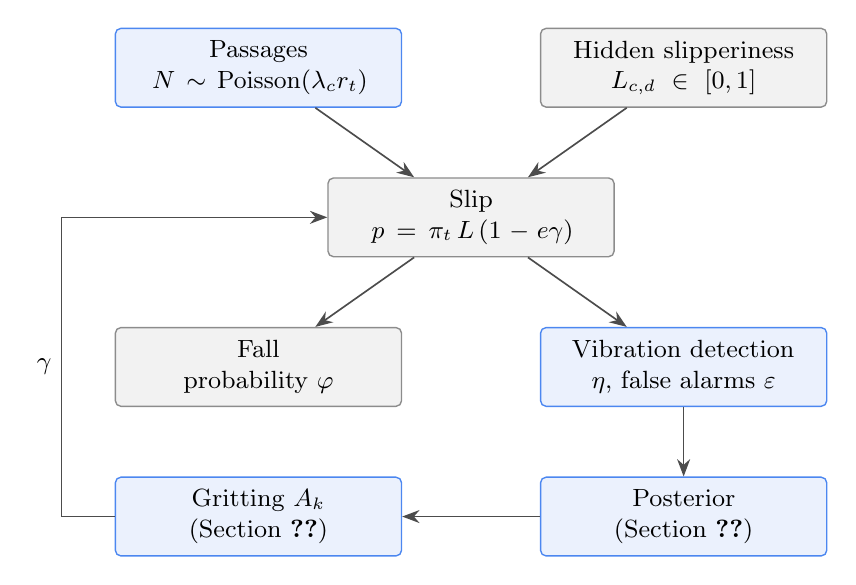
\begin{tikzpicture}[
  box/.style={draw,rounded corners=2pt,align=center,minimum height=10mm,text width=34mm,font=\small,line width=0.5pt},
  piilo/.style={box,fill=black!5,draw=black!45},
  nakyy/.style={box,fill=sininen!8,draw=sininen!70},
  nuoli/.style={-{Stealth[length=2.2mm]},line width=0.6pt,draw=black!70}]
  \node[nakyy] (N) at (0,0) {Passages\\ $N \sim \Poi(\lambda_c r_t)$};
  \node[piilo] (L) at (5.4,0) {Hidden slipperiness\\ $L_{c,d} \in [0,1]$};
  \node[piilo] (S) at (2.7,-1.9) {Slip\\ $p = \pi_t\, L\, (1 - e\gamma)$};
  \node[piilo] (F) at (0,-3.8) {Fall\\ probability $\varphi$};
  \node[nakyy] (D) at (5.4,-3.8) {Vibration detection\\ $\eta$, false alarms $\varepsilon$};
  \node[nakyy] (P) at (5.4,-5.7) {Posterior\\ (Section~\ref{sec:posteriori})};
  \node[nakyy] (A) at (0,-5.7) {Gritting $A_k$\\ (Section~\ref{sec:lauseet})};
  \draw[nuoli] (N) -- (S);
  \draw[nuoli] (L) -- (S);
  \draw[nuoli] (S) -- (F);
  \draw[nuoli] (S) -- (D);
  \draw[nuoli] (D) -- (P);
  \draw[nuoli] (P) -- (A);
  \draw[nuoli] (A.west) -- (-2.5,-5.7) -- node[midway,left,font=\small]{$\gamma$} (-2.5,-1.9) -- (S.west);
\end{tikzpicture}
\caption{Structure of the simulator in one square and one hour. Grey: hidden
truth. Blue: what the service sees and the decisions it makes. Gritting $\gamma$
reduces the slip risk in the following hours.}
\label{fig:malli}
\end{figure}

\subsection{Time and space}

Time advances in hours, $t \in \cT = \{1, \dots, T\}$, where $T = 744$ is the
number of hours in January 2026. Hour $t = 1$ is 00--01 on 1 January 2026,
Finnish time. The function $d(t)$ gives the local day of hour $t$; days change at
midnight.

The study area is a $300 \times 300$ metre square around the fire station (VPK
house) in Turku. It is divided into $10 \times 10$ metre squares. The model
contains the
\[
  |\cC| = 85
\]
squares that lie within 5 metres of one of four hand-drawn walking routes. The
crew works in larger units: $50 \times 50$ metre \emph{blocks}, of which there
are $|\cZ| = 20$. The map $\zeta\colon \cC \to \cZ$ assigns each square to its
block, and $\cC_z = \zeta^{-1}(z)$ is the set of squares in block $z$.

\subsection{Walking and weather}

The following quantities are deterministic and known to every policy.

\textbf{Base walking volume.} The hourly base volume $\lambda_c > 0$ of square
$c$ is the sum of the assumed hourly volumes of the routes passing near it. For a
block, $\lambda(z) = \sum_{c \in \cC_z} \lambda_c$.

\textbf{Daily rhythm.} Let $h_t$ be the clock hour at which hour $t$ starts.
Walking peaks in the morning and in the afternoon:
\[
  r_t = \Bigl(0.1 + 0.8\, e^{-((h_t - 8)/2)^2} + 0.9\, e^{-((h_t - 17)/3)^2}\Bigr)
  \cdot
  \begin{cases} 0.7 & \text{at weekends},\\ 1 & \text{on weekdays}. \end{cases}
\]

\textbf{Weather.} From the measured hourly means at Turku Artukainen (temperature
$T_t$, snow depth $s_t$, precipitation $q_t$) we compute the weather factor
\[
  w_t = 0.7 + 1.2 \cdot \1\{-3 \le T_t \le 1\} + 0.6 \cdot \1\{s_t > 0\}
        + 0.5 \cdot \1\{q_t > 0,\ T_t < 1\},
\]
which lies in $[0.7,\ 3.0]$. The base slip probability per passage is
$\pi_t = p_0 w_t$ with $p_0 = 0.01$.

The weather factor is an experimental rule of the simulator and has not been
calibrated against road-surface observations. It simply expresses that
pavements are more slippery around zero degrees than in hard frost.

\subsection{Hidden slipperiness}

Every square has, on every day, its own \emph{hidden slipperiness}
$L_{c,d} \in [0,1]$. It stands for things the weather does not tell: shade,
slope, water dripping from eaves, or polished ice. The value $L = 1$ is the most
slippery square possible and $L \approx 0$ is practically grippy.

We want a strongly skewed distribution: most squares are grippy, but a few are
really slippery. A Beta distribution $\Beta(a,b)$ with a small parameter $a$ has
this shape. For exact computation the distribution is discretised.

\begin{maaritelma}[Slipperiness levels]\label{maar:tasot}
Let $a, b > 0$ and $G \in \mathbb{N}$. Let $B \sim \Beta(a,b)$ with distribution
function $F$. Split $[0,1]$ into $G$ parts of equal probability at the points
$q_j = F^{-1}(j/G)$, $j = 0, \dots, G$, and set
\[
  \ell_g = \E\bigl[B \mid q_{g-1} < B \le q_g\bigr], \qquad g = 1, \dots, G.
\]
The slipperiness distribution is the uniform distribution on the levels,
$\nu = \frac{1}{G} \sum_{g=1}^{G} \delta_{\ell_g}$, with mean
$\mu = \sum_g \nu_g \ell_g$.
\end{maaritelma}

\begin{lemma}\label{le:tasot}
The levels of Definition~\ref{maar:tasot} satisfy:
\begin{enumerate}[(i)]
  \item $\ell_g = G \cdot \frac{a}{a+b} \bigl(I_{q_g}(a+1, b) - I_{q_{g-1}}(a+1, b)\bigr)$,
  where $I_x$ is the regularised incomplete beta function;
  \item $0 < \ell_1 < \ell_2 < \dots < \ell_G < 1$;
  \item $\mu = a/(a+b)$, i.e.\ the discretisation preserves the mean.
\end{enumerate}
\end{lemma}

\begin{proof}
The beta density satisfies $x f_{a,b}(x) = \frac{a}{a+b} f_{a+1,b}(x)$, because
$B(a+1,b)/B(a,b) = a/(a+b)$. Each interval has probability $1/G$, so
\[
  \ell_g = G \int_{q_{g-1}}^{q_g} x f_{a,b}(x)\,dx
         = G \frac{a}{a+b} \int_{q_{g-1}}^{q_g} f_{a+1,b}(x)\,dx,
\]
which is (i).

The density is positive on $(0,1)$. Hence $0 = q_0 < q_1 < \dots < q_G = 1$, and
the conditional mean of an interval lies strictly inside it:
$q_{g-1} < \ell_g < q_g$. This gives (ii).

Part (iii) is the law of total expectation:
$\mu = \sum_g \frac{1}{G}\, \E[B \mid \text{interval } g] = \E B = a/(a+b)$.
\end{proof}

\textbf{Default values.} The simulator uses $a = 1/4$, $b = 1$ and $G = 40$.
When $b = 1$ the distribution function is simply $F(x) = x^{a}$, and the levels
have the closed form
\[
  \ell_g = \frac{g^5 - (g-1)^5}{5\, G^4}.
\]
The mean is $\mu = 0.2$, the most slippery level is $\ell_{40} \approx 0.951$ and
the grippiest $\ell_1 \approx 7.8 \cdot 10^{-8}$. For the continuous distribution,
$\P(B < 0.004) \approx 0.25$ and $\P(B > 0.5) \approx 0.16$.

\begin{intuitio}
A quarter of the squares are practically grippy, and one in six is very
slippery. Such a world rewards targeting: if you knew where the slippery squares
were, gritting them would be many times as effective.
\end{intuitio}

Slipperiness changes daily. The persistence parameter $\rho$ says how likely
yesterday's state is to remain.

\begin{maaritelma}[Dynamics of slipperiness]\label{maar:dynamiikka}
Let $\rho \in [0, 1]$. For every square $c$ draw $L_{c,1} \sim \nu$. On the next
day $L_{c,d+1} = L_{c,d}$ with probability $\rho$; otherwise $L_{c,d+1}$ is
redrawn from $\nu$. All draws are independent across squares and days.
\end{maaritelma}

\begin{lemma}\label{le:markov}
For all $c$, $d$ and $j \ge 0$ we have $L_{c,d} \sim \nu$ and
\[
  \E[L_{c,d+j} \mid L_{c,1}, \dots, L_{c,d}] = \mu + \rho^j (L_{c,d} - \mu).
\]
\end{lemma}

\begin{proof}
The transition kernel is $P(\ell_g, \ell_h) = \rho\, \1\{g = h\} + (1-\rho)\nu_h$.
Since $\nu P = \rho \nu + (1-\rho)\nu = \nu$ and the initial distribution is
$\nu$, induction gives $L_{c,d} \sim \nu$ for all $d$. By the Markov property,
$\E[L_{c,d+1} \mid L_{c,\le d}] = \rho L_{c,d} + (1-\rho)\mu$, and the claim
follows by induction on $j$.
\end{proof}

The simulator's default is $\rho = 0$: every square's slipperiness is redrawn
each day. Then the previous day's detections are of no use, and the service has
to learn each day's situation from that day's detections.

\subsection{Passages, slips and detections}

All randomness is built on a single probability space so that independence
statements are precise.

\begin{maaritelma}[Probability space]\label{maar:avaruus}
The probability space $(\Omega, \cA, \P)$ carries the following mutually
independent families of random variables:
\begin{enumerate}[(a)]
  \item passages $N_{c,t} \sim \Poi(\lambda_c r_t)$, independent over all $(c,t)$;
  \item the slipperiness draws of Definition~\ref{maar:dynamiikka};
  \item per-passage uniform variables $U_{c,t,i,j}$ with $i \in \mathbb{N}$ and
  $j \in \{1, 2, 3\}$;
  \item an optional randomisation $V$ of a blind policy (Definition~\ref{maar:politiikka}).
\end{enumerate}
Write $\Psi_t = (N_{c,t}, U_{c,t,i,j})_{c, i, j}$ for the randomness of hour $t$
and $L$ for the whole slipperiness process. Then $L, V, \Psi_1, \Psi_2, \dots$ are
independent.
\end{maaritelma}

Let $\gamma_{c,t} \in \{0,1\}$ indicate whether the block of square $c$ is
gritted in hour $t$; it is determined by the policy (Section~\ref{sec:huolto}).
The remaining parameters of the model are
\begin{center}
\begin{tabular}{@{}ll@{}}
$e \in [0,1]$ & effect of gritting, \\
$\varphi$ & probability that a slip becomes a fall, \\
$\eta$ & sensitivity of the detector, \\
$\varepsilon$ & probability of a false alarm per passage.
\end{tabular}
\end{center}

The slip probability per passage is
\begin{equation}\label{eq:p}
  p_{c,t} = \pi_t\, L_{c,d(t)}\, (1 - e\,\gamma_{c,t}).
\end{equation}
We assume $\pi_t \ell_G < 1$ for all $t$; with the default values
$\max_t \pi_t \ell_G \le 0.03 \cdot 0.951$.

Each passage $i = 1, \dots, N_{c,t}$ is treated separately:
\begin{itemize}
  \item the passage leads to a slip if $U_{c,t,i,1} \le p_{c,t}$;
  \item a slip leads to a fall if $U_{c,t,i,2} \le \varphi$;
  \item the detector raises an alarm if a slip occurred and $U_{c,t,i,3} \le \eta$,
  or if no slip occurred and $U_{c,t,i,3} \le \varepsilon$.
\end{itemize}
The numbers of slips, falls and detections are denoted $S_{c,t}$, $F_{c,t}$ and
$D_{c,t}$.

\begin{lemma}[Distribution of detections and falls]\label{le:havainnot}
Let $\cG_t = \sigma(L, V, \Psi_1, \dots, \Psi_{t-1}, N_{\cdot,t})$, and let
$\gamma_{\cdot,t}$ be $\sigma(L, V, \Psi_{<t})$-measurable. Then, conditionally on
$\cG_t$, the variables $D_{c,t}$, $c \in \cC$, are independent and
\[
  D_{c,t} \sim \Bin\bigl(N_{c,t},\, \theta_t(L_{c,d(t)}, \gamma_{c,t})\bigr),
  \qquad
  \theta_t(\ell, \gamma) = \varepsilon + (\eta - \varepsilon)\, \pi_t\, \ell\, (1 - e \gamma).
\]
Moreover $\E[F_{c,t} \mid \cG_t] = \varphi\, N_{c,t}\, p_{c,t}$.
\end{lemma}

\begin{proof}
Conditionally on $\cG_t$ the probability $p_{c,t}$ is known, and the variables
$U_{c,t,\cdot,\cdot}$ are independent of $\cG_t$. A single passage raises an alarm
with probability
$p_{c,t}\eta + (1 - p_{c,t})\varepsilon = \theta_t(L_{c,d(t)}, \gamma_{c,t})$, and
passages are independent of each other. Likewise a passage leads to a fall with
probability $p_{c,t}\varphi$.
\end{proof}

\begin{intuitio}
The alarm probability $\theta$ is an \emph{affine} function of slipperiness. When
$\eta > \varepsilon$, a more slippery square produces more alarms per passage on
average. This is the only channel through which the service learns anything
about slipperiness.
\end{intuitio}

\begin{huomautus}[Implementation and common random numbers]\label{hu:crn}
The code does not draw every passage separately. It draws the totals $S$, $F$
and $D$ directly from binomial distributions by inversion, and every policy
receives the same uniform random number. Conditionally on $(N_{c,t}, p_{c,t})$ the
totals have the same distribution as above, so each policy's own distribution is
exactly this model. The common random numbers couple the policies only so that
their difference can be estimated with lower variance.
\end{huomautus}

\subsection{Gritting and the no-overlap rule}\label{sec:huolto}

\begin{maaritelma}[Gritting rounds]\label{maar:huolto}
Let $\Delta$, $H$ and $K$ be positive integers: the gritting interval, the
duration of the effect and the number of blocks gritted per round. Rounds start
at hours $\tau_k = 1 + (k-1)\Delta$, $k = 1, \dots, \kappa$, where
$\kappa = \lceil T/\Delta \rceil$. The \emph{effect window} of round $k$ is
\[
  W_k = \{\tau_k, \dots, \tau_k + H - 1\} \cap \cT.
\]
In round $k$ a set $A_k \subseteq \cZ$ with $|A_k| = K$ is chosen, only among
eligible blocks:
\[
  A_k \subseteq E_k := \cZ \setminus \bigcup\bigl\{A_j : j < k,\ \tau_j + H > \tau_k\bigr\}.
\]
This is the \emph{no-overlap rule}: a block is not chosen while its previous
gritting is still in effect. The gritting indicator is
$\gamma_{c,t} = \1\{\exists k : \zeta(c) \in A_k,\ t \in W_k\}$.
\end{maaritelma}

\begin{lemma}\label{le:erilliset}
Under the no-overlap rule, the effect windows of the same block are disjoint.
Hence
\[
  \gamma_{c,t} = \sum_{k} \1\{\zeta(c) \in A_k\}\, \1\{t \in W_k\}.
\]
\end{lemma}

\begin{proof}
Let $j < k$ and $z \in A_j \cap A_k$. By eligibility $\tau_j + H \le \tau_k$, so
$\max W_j < \tau_k = \min W_k$. The sum therefore has at most one nonzero term.
\end{proof}

\subsection{Information, policies and objective}

The service sees passages and vibration detections as they happen. Its
information at the end of hour $t$ is
\[
  \cF_t = \sigma\bigl(N_{c,s},\, D_{c,s} : c \in \cC,\ s \le t\bigr),
\]
and $\cF_0$ is trivial.

\begin{maaritelma}[Policy]\label{maar:politiikka}
A \emph{policy} is a rule whose choice $A_k$ is $\cF_{\tau_k - 1}$-measurable and
eligible: the decision is made before the round starts, using all information
gathered so far. Because detections depend on earlier gritting, the information
depends on the policy; when needed we write $\cF^\pi_t$.
\begin{itemize}
  \item A policy is \emph{blind} if $A_k$ is measurable with respect to
  $\cB_{\tau_k - 1} \vee \sigma(V)$, where $\cB_t = \sigma(N_{c,s} : s \le t)$.
  A blind policy may use the clock, the weather, passages and its own
  randomisation, but not vibration detections.
  \item The \emph{oracle} has the information
  $\cH_k = \sigma\bigl(L_{\cdot,d} : d \le d(\tau_k);\ \Psi_s : s < \tau_k\bigr)$.
  It knows the current day's slipperiness but not future randomness. For every
  policy, $\cF^\pi_{\tau_k - 1} \subseteq \cH_k$.
\end{itemize}
\end{maaritelma}

\begin{maaritelma}[Objective]
The value of a policy $\pi$ is the expected number of falls
\[
  J(\pi) = \E^\pi\Bigl[\sum_{c \in \cC} \sum_{t \in \cT} F_{c,t}\Bigr].
\]
\end{maaritelma}

The simulator's column \texttt{expected\_falls} is
$\sum_{c,t} \varphi N_{c,t} p_{c,t}$. By Lemma~\ref{le:havainnot} and the tower
property its expectation is $J(\pi)$. It is therefore an unbiased estimator with
lower variance than the drawn falls.

\begin{table}[ht]
\centering
\small
\begin{tabular}{@{}l l@{}}
\toprule
Symbol & Meaning \\
\midrule
$c \in \cC$, $z \in \cZ$ & square ($10 \times 10$ m) and block ($50 \times 50$ m) \\
$t$, $d(t)$ & hour and its day \\
$\lambda_c$, $r_t$, $\pi_t$ & base walking volume, daily rhythm, weather-driven base risk \\
$L_{c,d}$, $\ell_g$, $\nu$, $\mu$ & hidden slipperiness, its levels, distribution and mean \\
$\rho$ & day-to-day persistence of slipperiness \\
$N$, $S$, $F$, $D$ & passages, slips, falls, vibration detections \\
$e$, $\varphi$, $\eta$, $\varepsilon$ & gritting effect, fall share, sensitivity, false alarms \\
$\Delta$, $H$, $K$ & gritting interval, effect duration, blocks per round \\
$A_k$, $W_k$, $\gamma_{c,t}$ & round choice, effect window, gritting indicator \\
$\cF_t$, $\cB_t$, $\cH_k$ & information of the service, a blind policy and the oracle \\
$J(\pi)$ & expected number of falls \\
\bottomrule
\end{tabular}
\caption{Main notation.}
\label{tab:merkinnat}
\end{table}

% ---------------------------------------------------------------------------
\section{What the service knows: the beta-binomial posterior}\label{sec:posteriori}

The service does not see slipperiness, but it can infer it from detections with
Bayes' rule. This section shows that the inference splits square by square and
can be computed with a simple recursion.

Assume the policy is \emph{deterministic}: the choice $A_k$ is a deterministic
function of the observation history. All policies in the code are, with ties
broken by block number.

\begin{propositio}[Filter]\label{pr:suodin}
Conditionally on $\cF_t$, the slipperiness chains $(L_{c,d})_d$, $c \in \cC$, are
independent. The filtering distribution of each square,
\[
  w_{c,g}(t) = \P\bigl(L_{c,d(t)} = \ell_g \mid \cF_t\bigr),
\]
follows the recursion:
\begin{enumerate}[(i)]
  \item Initially $w_c = \nu$. When the day changes, the distribution is
  predicted for the next day: $w_c \mapsto \rho\, w_c + (1 - \rho)\nu$.
  \item The detections of hour $t$ update the distribution:
  \[
    w_{c,g}(t) \;\propto\; w_{c,g}(t-1)\; \theta_t(\ell_g, \gamma_{c,t})^{D_{c,t}}
    \bigl(1 - \theta_t(\ell_g, \gamma_{c,t})\bigr)^{N_{c,t} - D_{c,t}}.
  \]
\end{enumerate}
The posterior mean of slipperiness is $m_c(t) = \sum_g w_{c,g}(t)\, \ell_g$.
\end{propositio}

\begin{proof}
Let $h = (n_{c,s}, \delta_{c,s})_{c \in \cC,\, s \le t}$ be an observation
history and $l = (l_{c,d})$ a slipperiness path. Since the policy is
deterministic, $\gamma_{c,s} = \gamma_{c,s}(h_{<s})$. Conditioning hour by hour
with Lemma~\ref{le:havainnot} gives
\[
  \P(N_{\le t} = n,\ D_{\le t} = \delta \mid L = l)
  = \prod_{s \le t} \prod_{c} \Poi(n_{c,s}; \lambda_c r_s)
    \binom{n_{c,s}}{\delta_{c,s}}\, \theta_s^{\delta_{c,s}} (1 - \theta_s)^{n_{c,s} - \delta_{c,s}},
\]
where $\theta_s = \theta_s\bigl(l_{c,d(s)}, \gamma_{c,s}(h_{<s})\bigr)$.

As a function of the path $l$ this is a product of per-square factors. The prior
is also a product, because the chains of different squares are independent.
Hence the posterior is a product, and the posterior of each square is that of a
hidden Markov model. Its transition kernel is $P$ from Lemma~\ref{le:markov}, and
the probability of an hour's observation is the binomial factor above. The
forward algorithm gives (i) and (ii); the prediction in (i) is
$wP = \rho w + (1 - \rho)\nu$.
\end{proof}

In the code the update is the function \texttt{paivita\_posteriori}. The
simulator draws slipperiness from the same discrete distribution $\nu$ that the
service uses as its prior, so the computed posterior is exact, not an
approximation.

The name \emph{beta-binomial} comes from the following special case, in which the
prior is a continuous beta distribution and an alarm reveals slipperiness
directly.

\begin{propositio}[Conjugate special case]\label{pr:konjugaatti}
Let the prior be the continuous $\Beta(a,b)$ and let $\theta = \ell$, i.e.\
$\eta = 1$, $\varepsilon = 0$ and $\pi_s(1 - e\gamma) = 1$. If during one day there
are $n = \sum_s N_s$ passages and $y = \sum_s D_s$ detections, the posterior is
$\Beta(a + y,\ b + n - y)$, and
\[
  \E[L \mid \text{data}] = \frac{a + y}{a + b + n}
  = \underbrace{\frac{a + b}{a + b + n}}_{\text{weight of prior}}\cdot\frac{a}{a+b}
  \;+\; \underbrace{\frac{n}{a + b + n}}_{\text{weight of data}}\cdot\frac{y}{n}.
\]
Moreover, the marginal distribution of $y$ given $n$ is the beta-binomial
distribution $\mathrm{BB}(n, a, b)$.
\end{propositio}

\begin{proof}
The posterior density is proportional to
$\ell^{a-1}(1-\ell)^{b-1} \cdot \ell^{y}(1-\ell)^{n-y}$, which is the kernel of the
$\Beta(a+y, b+n-y)$ density. The marginal is
$\binom{n}{y} B(a+y, b+n-y)/B(a,b)$, which is the definition of the beta-binomial
distribution.
\end{proof}

\begin{intuitio}
The prior $\Beta(a,b)$ is worth $a + b$ imaginary passages, $a$ of which raised
an alarm. The posterior mean is a weighted average: with little data it stays
near the prior mean, with much data it approaches the observed share $y/n$. A
single alarm from a single passage does not make a square slippery.

In the simulator $\theta$ is an affine function of slipperiness, so the posterior
is not of beta form. It is therefore computed exactly on the grid of levels
$\ell_1, \dots, \ell_G$. The check \texttt{tarkista\_tammikuu.R} verifies that the
grid computation reproduces Proposition~\ref{pr:konjugaatti} when $G = 4000$.
\end{intuitio}

% ---------------------------------------------------------------------------
\section{Decomposing the value of gritting}\label{sec:hajotelma}

The number of falls in a month is a complicated random variable: every gritting
affects future slips, detections and decisions. This section shows that its
expectation nevertheless splits neatly into one term per gritting round.

Define the \emph{risk mass} of block $z$ in the effect window of round $k$ and
its deterministic counterpart, the \emph{exposure}:
\[
  R_{z,k} = \sum_{c \in \cC_z} \sum_{t \in W_k} N_{c,t}\, \pi_t\, L_{c,d(t)},
  \qquad
  \Lambda_{z,k} = \lambda(z)\, \kappa_k, \quad \kappa_k = \sum_{t \in W_k} r_t \pi_t .
\]
The risk mass is the amount of slip risk that gritting could remove. It does not
depend on the policy, because it is a function of passages and slipperiness only.

\begin{propositio}[Decomposition]\label{pr:hajotelma}
Let $\cG_k$ be any $\sigma$-algebra with respect to which $A_k$ is measurable.
For every policy that respects the no-overlap rule,
\[
  J(\pi) = \mathsf{B} - e \varphi \sum_{k=1}^{\kappa}
  \E^\pi\Bigl[\sum_{z \in A_k} \E[R_{z,k} \mid \cG_k]\Bigr],
  \qquad
  \mathsf{B} = \varphi \mu \sum_{c,t} \lambda_c r_t \pi_t = J(\pol{no-grit}).
\]
\end{propositio}

\begin{proof}
\emph{Step 1.} By Lemma~\ref{le:havainnot} and the tower property,
$\E F_{c,t} = \varphi\,\E\bigl[N_{c,t}\, \pi_t L_{c,d(t)} (1 - e\gamma_{c,t})\bigr]$.

\emph{Step 2.} By Lemma~\ref{le:erilliset} the gritted part can be grouped by
round:
\[
  \sum_{c,t} N_{c,t}\pi_t L_{c,d(t)} \gamma_{c,t}
  = \sum_k \sum_{z \in A_k} \sum_{c \in \cC_z} \sum_{t \in W_k} N_{c,t}\pi_t L_{c,d(t)}
  = \sum_k \sum_{z \in A_k} R_{z,k}.
\]

\emph{Step 3.} Since $N \perp L$ and $L_{c,d} \sim \nu$,
$\E[N_{c,t}\pi_t L_{c,d(t)}] = \lambda_c r_t \pi_t \mu$, which gives $\mathsf{B}$.

\emph{Step 4.} Finally
$\E[\1\{z \in A_k\} R_{z,k}] = \E\bigl[\1\{z \in A_k\}\,\E[R_{z,k} \mid \cG_k]\bigr]$,
because $\1\{z \in A_k\}$ is $\cG_k$-measurable and $R_{z,k} \ge 0$ is integrable.
\end{proof}

\begin{intuitio}
The no-overlap rule guarantees that no square-hour ever benefits from two
grittings. The value of a policy is then a sum over rounds: how much risk mass
the chosen blocks contain \emph{in the light of the information available when
choosing}. The best policy is the one that can pick the blocks with the largest
risk mass.
\end{intuitio}

The next lemma says what ``the information available when choosing'' amounts to
for the different policies.

\begin{lemma}[Conditional risk mass]\label{le:ehdollinen}
Let $\cG \subseteq \sigma(L, V, \Psi_{<\tau_k})$ and $m_{c,d} = \E[L_{c,d} \mid \cG]$.
Then
\[
  \E[R_{z,k} \mid \cG] = \sum_{c \in \cC_z} \lambda_c \sum_{t \in W_k} r_t \pi_t\, m_{c,d(t)}.
\]
In particular:
\begin{enumerate}[(i)]
  \item for the service ($\cG = \cF^\pi_{\tau_k - 1}$), $m_{c,d}$ is the posterior
  mean of Proposition~\ref{pr:suodin};
  \item for a blind policy ($\cG = \cB_{\tau_k-1} \vee \sigma(V)$),
  $m_{c,d} = \mu$, so $\E[R_{z,k} \mid \cG] = \mu \Lambda_{z,k}$;
  \item for the oracle ($\cG = \cH_k$),
  $m_{c,d} = \mu + \rho^{d - d(\tau_k)}(L_{c,d(\tau_k)} - \mu)$ for $d \ge d(\tau_k)$.
\end{enumerate}
\end{lemma}

\begin{proof}
For $t \ge \tau_k$ the passage count $N_{c,t}$ belongs to the randomness $\Psi_t$
and is therefore independent of $\sigma(L, V, \Psi_{<\tau_k})$, which contains
$\cG \vee \sigma(L)$. Hence
$\E[N_{c,t} L_{c,d(t)} \mid \cG] = \E[N_{c,t}]\,\E[L_{c,d(t)} \mid \cG]$.

In (ii), $L$ is independent of $N$ and $V$, so
$\E[L_{c,d} \mid \cG] = \E L_{c,d} = \mu$. Part (iii) follows from
Lemma~\ref{le:markov}, because the draws of future days are independent of
$\cH_k$.
\end{proof}

% ---------------------------------------------------------------------------
\section{Main results}\label{sec:lauseet}

\subsection{Assumptions and policies}

Two assumptions make the rounds independent selection problems.

\begin{oletus}[No carry-over]\label{ol:A}
$H \le \Delta$: the effect of gritting ends no later than the start of the next round.
\end{oletus}

\begin{oletus}[Window within one day]\label{ol:B}
For every $k$ and every $t \in W_k$ we have $d(t) = d(\tau_k)$.
\end{oletus}

Under Assumption~\ref{ol:A}, $\tau_j + H \le \tau_k$ whenever $j < k$. Then
$E_k = \cZ$: every set of $K$ blocks is eligible, and earlier choices do not
restrict later ones.

The simulator's defaults are $\Delta = H = 6$ and $K = 2$. Since 6 divides 24,
the first round starts at midnight and January has no daylight-saving change,
Assumption~\ref{ol:B} also holds.

\begin{maaritelma}[Policies of the simulator]\label{maar:koodi}
Write $\cA_K = \{A \subseteq \cZ : |A| = K\}$.
\begin{itemize}
  \item \pol{no-grit}: no gritting, $\gamma \equiv 0$.
  \item \pol{rotation}: the next $K$ eligible blocks in cyclic order.
  \item \pol{busiest}: $A_k \in \argmax_{A \in \cA_K} \sum_{z \in A} \Lambda_{z,k}$,
  i.e.\ the $K$ blocks with the largest $\lambda(z)$.
  \item \pol{pito}: $A_k \in \argmax_{A \in \cA_K} \sum_{z \in A} \hat S_{z,k}$,
  where $\hat S_{z,k} = \E[R_{z,k} \mid \cF^{\pol{pito}}_{\tau_k - 1}]$.
  \item \pol{oracle}: $A_k \in \argmax_{A \in \cA_K} \sum_{z \in A} \E[R_{z,k} \mid \cH_k]$.
\end{itemize}
\end{maaritelma}

\subsection{The best blind policy}

\begin{lause}[Best blind policy]\label{la:sokea}
Under Assumption~\ref{ol:A}, every blind policy $\beta$ satisfies
\[
  J(\beta) \;\ge\; J^\ast_{\mathrm{blind}} := \mathsf{B} - e\varphi\mu \sum_{k} \max_{A \in \cA_K} \sum_{z \in A} \Lambda_{z,k}
  \;=\; J(\pol{busiest}).
\]
\end{lause}

\begin{proof}
Take $\cG_k = \cB_{\tau_k - 1} \vee \sigma(V)$ in Proposition~\ref{pr:hajotelma}.
By Lemma~\ref{le:ehdollinen}~(ii),
\[
  J(\beta) = \mathsf{B} - e\varphi\mu \sum_k \E\Bigl[\sum_{z \in A_k} \Lambda_{z,k}\Bigr].
\]
Since $A_k \in \cA_K$, the sum is at most the maximum. The policy \pol{busiest}
attains the maximum in every round. Since $\Lambda_{z,k} = \lambda(z)\kappa_k$ and
$\kappa_k > 0$, the maximising set consists of the $K$ blocks with the largest
$\lambda(z)$.
\end{proof}

\begin{seuraus}
$J(\pol{rotation}) \ge J(\pol{busiest})$. The same holds for every rule that
chooses blocks by clock, weather or observed passages.
\end{seuraus}

\begin{intuitio}
Without vibration detections, the best estimate of every square's slipperiness
is the mean $\mu$. The value of gritting is then proportional to exposure alone,
and the best blind rule is to grit the busiest blocks. Observed passages say
nothing about slipperiness, because passages and slipperiness are independent in
the model.
\end{intuitio}

\subsection{The value of vibration detections}

\begin{lause}[Value of detections]\label{la:arvo}
Under Assumption~\ref{ol:A}, $J(\pol{pito}) \le J^\ast_{\mathrm{blind}}$, so
$J(\pol{pito}) \le J(\beta)$ for every blind policy $\beta$. More precisely,
\begin{equation}\label{eq:arvo}
  J(\pol{busiest}) - J(\pol{pito}) = e\varphi \sum_{k} \E\Bigl[\max_{A \in \cA_K} \sum_{z \in A} \hat S_{z,k}
  - \sum_{z \in A^{\pol{busiest}}_k} \hat S_{z,k}\Bigr] \;\ge\; 0,
\end{equation}
where every term inside the expectation is pointwise non-negative.
\end{lause}

\begin{proof}
Take $\cG_k = \cF^{\pol{pito}}_{\tau_k - 1}$ in Proposition~\ref{pr:hajotelma}.
Since \pol{pito} maximises,
\[
  J(\pol{pito}) = \mathsf{B} - e\varphi \sum_k \E\Bigl[\max_{A \in \cA_K}\sum_{z \in A}\hat S_{z,k}\Bigr].
\]
The set $A^{\pol{busiest}}_k$ is deterministic and
$\E \hat S_{z,k} = \E R_{z,k} = \mu \Lambda_{z,k}$. Hence
\[
  \E\Bigl[\sum_{z \in A^{\pol{busiest}}_k} \hat S_{z,k}\Bigr] = \mu \max_{A \in \cA_K}\sum_{z \in A}\Lambda_{z,k}.
\]
Subtracting gives~\eqref{eq:arvo}. Each term is non-negative because the maximum
is at least the value of the sum on any set, in particular on
$A^{\pol{busiest}}_k$.
\end{proof}

\begin{intuitio}
A service that uses detections can always pick the same set as the best blind
rule. It deviates only when the posterior promises more risk mass. The posterior
mean equals the prior on average, so the deviations cannot make the choice worse
on average. This is the basic value-of-information result $\E \max \ge \max \E$.
\end{intuitio}

\subsection{The oracle}

\begin{lause}[Oracle]\label{la:oraakkeli}
Under Assumption~\ref{ol:A}, $J(\pol{oracle}) \le J(\pi)$ for every policy $\pi$.
In particular $J(\pol{oracle}) \le J(\pol{pito})$.
\end{lause}

\begin{proof}
Since $\cF^\pi_{\tau_k - 1} \subseteq \cH_k$, the set $A^\pi_k$ is
$\cH_k$-measurable. By Proposition~\ref{pr:hajotelma},
\[
  J(\pi) = \mathsf{B} - e\varphi\sum_k \E\Bigl[\sum_{z \in A^\pi_k}\E[R_{z,k}\mid\cH_k]\Bigr].
\]
The inner sum is at most
$\max_{A \in \cA_K}\sum_{z \in A}\E[R_{z,k}\mid\cH_k]$, which the oracle attains.
\end{proof}

\subsection{When the gain is strict}

Theorem~\ref{la:arvo} says that detections do no harm. The next theorem says
when they genuinely help.

\begin{lause}[Strict gain]\label{la:aito}
Assume Assumptions~\ref{ol:A} and~\ref{ol:B} and the following conditions.
\begin{enumerate}[label=(C\arabic*),leftmargin=3.2em]
  \item \emph{Discrimination:} $0 < \varepsilon < \eta \le 1$, $0 < e < 1$ and $\varphi > 0$.
  \item \emph{Variation:} $G \ge 2$.
  \item \emph{Room to choose:} $K < |\cZ|$, $\Delta < 24$, and there are blocks
  $z^\ast \in A^{\pol{busiest}}_2$ and $z' \notin A^{\pol{busiest}}_2$ with
  $\ell_G\, \lambda(z') > \ell_1\, \lambda(z^\ast)$.
\end{enumerate}
Then $J(\pol{pito}) < J(\pol{busiest})$.
\end{lause}

\begin{proof}
The terms of~\eqref{eq:arvo} are non-negative and $e\varphi > 0$. It therefore
suffices to show that in round $k = 2$, with positive probability,
\begin{equation}\label{eq:aito}
  \max_{A \in \cA_K}\sum_{z \in A}\hat S_{z,2} \;>\; \sum_{z \in A^{\pol{busiest}}_2}\hat S_{z,2}.
\end{equation}

\emph{Step 1: a swap is enough.} Since $\Delta < 24$, round $\tau_2 = 1 + \Delta$
falls on the first day. By Assumption~\ref{ol:B} and Lemma~\ref{le:ehdollinen},
\[
  \hat S_{z,2} = \kappa_2 \sum_{c \in \cC_z}\lambda_c m_c,
  \qquad m_c = \E[L_{c,1} \mid \cF_{\Delta}],\quad \kappa_2 > 0.
\]
If $\sum_{c \in \cC_{z'}}\lambda_c m_c > \sum_{c \in \cC_{z^\ast}}\lambda_c m_c$,
the set $(A^{\pol{busiest}}_2 \setminus\{z^\ast\}) \cup \{z'\}$ gives a strictly
larger sum, and~\eqref{eq:aito} holds.

\emph{Step 2: extreme but possible data.} Let $n \in \mathbb{N}$ and let $E_n$ be
the event that every square $c \in \cC_{z'} \cup \cC_{z^\ast}$ has $N_{c,1} = n$ and
$N_{c,s} = 0$ for $2 \le s \le \Delta$, while $D_{c,1} = n$ on the squares of $z'$
and $D_{c,1} = 0$ on the squares of $z^\ast$. Since $\lambda_c r_s > 0$, and by (C1)
and $\pi_t\ell_G < 1$ we have $0 < \varepsilon \le \theta_1(\ell, \gamma) < 1$,
Lemma~\ref{le:havainnot} gives $\P(E_n) > 0$.

\emph{Step 3: the posterior concentrates.} On $E_n$, Proposition~\ref{pr:suodin}
gives on the first day
\[
  w_{c,g} = \frac{\theta_1(\ell_g,\gamma_c)^n}{\sum_h \theta_1(\ell_h,\gamma_c)^n}
  \quad (c \in \cC_{z'}),
  \qquad
  w_{c,g} = \frac{(1-\theta_1(\ell_g,\gamma_c))^n}{\sum_h (1-\theta_1(\ell_h,\gamma_c))^n}
  \quad (c \in \cC_{z^\ast}),
\]
because the prior is uniform and the hours $s \ge 2$ contain no passages. By (C1),
(C2) and Lemma~\ref{le:tasot}~(ii), $\theta_1(\ell, \gamma)$ is strictly
increasing in $\ell$ for both $\gamma \in \{0, 1\}$. As $n \to \infty$ the
weights concentrate on level $G$ in block $z'$ and on level $1$ in block
$z^\ast$. Hence
\[
  \sum_{c \in \cC_{z'}}\lambda_c m_c - \sum_{c \in \cC_{z^\ast}}\lambda_c m_c
  \;\longrightarrow\; \ell_G\lambda(z') - \ell_1\lambda(z^\ast) \;>\; 0.
\]

\emph{Step 4: conclusion.} The limit does not depend on other data, because each
square's posterior depends only on its own observations. Choose $n$ large enough
for the difference to be positive on $E_n$. Then~\eqref{eq:aito} holds with
probability at least $\P(E_n) > 0$.
\end{proof}

The simulator's defaults satisfy the conditions: $\varepsilon = 0.0002 < \eta = 0.8$,
$e = 0.8$, $\varphi = 0.02$, $G = 40$, $K = 2 < 20$ and $\Delta = 6$. Moreover
$\ell_1/\ell_G \approx 8 \cdot 10^{-8}$, while the smallest $\lambda(z)$ is 16 and
the largest 157 passages per hour. Condition (C3) therefore holds for every pair
of blocks.

\begin{intuitio}
The proof builds one clear-cut situation: in the early morning a quiet block
produces nothing but alarms and a busy block none at all. The best blind rule
still grits the busy block, but the service knows better. Because the situation
has positive probability, the expected gain is strictly positive.
\end{intuitio}

\subsection{When there is no gain}

\begin{lause}[Necessary conditions]\label{la:valttamaton}
Under Assumption~\ref{ol:A}:
\begin{enumerate}[(i)]
  \item if $\eta = \varepsilon$, then $J(\pol{pito}) = J(\pol{busiest})$;
  \item if $G = 1$, then $J(\pol{oracle}) = J(\pol{pito}) = J(\pol{busiest})$;
  \item if $e = 0$ or $\varphi = 0$, then $J(\pi) = \mathsf{B}$ for every policy.
\end{enumerate}
\end{lause}

\begin{proof}
(i) When $\eta = \varepsilon$, the probability $\theta_t$ does not depend on
slipperiness, so the update of Proposition~\ref{pr:suodin} leaves the
distribution unchanged. Then $w(t) = \nu$ and $m_c = \mu$, so
$\hat S_{z,k} = \mu\Lambda_{z,k}$ is deterministic and the difference
in~\eqref{eq:arvo} is zero.

(ii) When $G = 1$, slipperiness is the constant $\mu$, and all three policies
score blocks by $\mu\Lambda_{z,k}$.

(iii) The coefficient of the gain term in Proposition~\ref{pr:hajotelma} is
$e\varphi = 0$.
\end{proof}

\subsection{Summary and remarks}

\begin{seuraus}[Ordering]\label{se:jarjestys}
Under Assumption~\ref{ol:A},
\[
  J(\pol{oracle}) \le J(\pol{pito}) \le J(\pol{busiest}) \le J(\pol{rotation}) \le J(\pol{no-grit}) = \mathsf{B}.
\]
Under the conditions of Theorem~\ref{la:aito}, the second inequality is strict.
\end{seuraus}

\begin{huomautus}[Longer effect]\label{hu:H}
When $H > \Delta$, Lemma~\ref{le:erilliset} and Proposition~\ref{pr:hajotelma}
still hold thanks to the no-overlap rule. The eligible sets $E_k$, however,
depend on earlier choices, so the proofs do not carry over as such. A choice
based on detections may, for example, take a block out of use at a moment when a
blind rule would have used it. The code allows this setting, but its results in
Table~\ref{tab:herkkyys} are empirical only.
\end{huomautus}

\begin{huomautus}[Greediness]
\pol{pito} maximises the conditional gain of each round separately. The theorems
do not claim it is optimal among all policies that use detections. Gritting
weakens a block's future detections, since $\theta$ shrinks by the factor
$(1-e)$, so a more exploratory policy could do better. The proof of
Theorem~\ref{la:arvo} nevertheless applies verbatim to any policy that chooses
$\argmax_A \sum_{z\in A}\E[R_{z,k} \mid \cG_k]$ for some $\sigma$-algebra
$\cG_k \subseteq \cH_k$.
\end{huomautus}

% ---------------------------------------------------------------------------
\section{Correspondence between code and model}\label{sec:koodi}

The code is in Finnish. Table~\ref{tab:parametrit} shows where each symbol
lives in the code, and Table~\ref{tab:politiikat} maps the policy names of this
paper to the code's identifiers. The files are in \texttt{If/labra/v0}.

\begin{table}[ht]
\centering
\small
\begin{tabular}{@{}lll@{}}
\toprule
Symbol & In the code & Default \\
\midrule
$a, b, G$ & \texttt{liukkaus\_a}, \texttt{liukkaus\_b}, \texttt{liukkaustasoja} & $0.25$; $1$; $40$ \\
$\rho$ & \texttt{pysyvyys} & $0$ \\
$p_0$ & \texttt{liukastuminen\_p} & $0.01$ \\
$\varphi$ & \texttt{kaatuminen\_liukastumisesta\_p} & $0.02$ \\
$\eta, \varepsilon$ & \texttt{tunnistus\_p}, \texttt{virhehavainto\_p} & $0.8$; $0.0002$ \\
$\Delta, H, K$ & \texttt{huoltovali\_h}, \texttt{huollon\_kesto\_h}, \texttt{huoltokohteita} & $6$; $6$; $2$ \\
$e$ & \texttt{huollon\_teho} & $0.8$ \\
$\ell_g$ & \texttt{liukkaustasot()} & Lemma~\ref{le:tasot} \\
$w_{c,g}$ & \texttt{exp(logw)}, \texttt{paivita\_posteriori()} & Proposition~\ref{pr:suodin} \\
$w_t$, $r_t$ & \texttt{saakerroin()}, \texttt{rytmi} & Section~\ref{sec:malli} \\
\bottomrule
\end{tabular}
\caption{Notation of the paper and variables of the simulator
(\texttt{tammikuu\_asetukset.R}, \texttt{R/simuloi\_tammikuu.R}).}
\label{tab:parametrit}
\end{table}

\begin{table}[ht]
\centering
\small
\begin{tabular}{@{}lll@{}}
\toprule
This paper & Code identifier & Meaning \\
\midrule
\pol{no-grit} & \texttt{ei\_huoltoa} & no gritting \\
\pol{rotation} & \texttt{aikataulu} & fixed rotation \\
\pol{busiest} & \texttt{kulku} & busiest blocks, best blind policy \\
\pol{pito} & \texttt{tuote} & detection-based targeting (the product) \\
\pol{oracle} & \texttt{oraakkeli} & knows the hidden slipperiness \\
\bottomrule
\end{tabular}
\caption{Policy names in this paper and in the code.}
\label{tab:politiikat}
\end{table}

The code scores block $z$ in round $k$ by
\[
  \mathrm{score}(z) = \sum_{c \in \cC_z}\lambda_c\bigl(\mu A_0 + (m_c - \mu)A_1\bigr),
  \qquad A_0 = \sum_{t \in W_k} r_t,\quad A_1 = \sum_{t \in W_k} r_t\,\rho^{d(t) - d(\tau_k)}.
\]
Here $m_c = \mu$ for \pol{busiest}, the posterior mean for \pol{pito}, and
$L_{c,d(\tau_k)}$ for \pol{oracle}. The weather factor is left out so that the
decision does not need future weather.

\begin{propositio}
Under Assumptions~\ref{ol:A} and~\ref{ol:B}, the code's \pol{busiest},
\pol{pito} and \pol{oracle} choose an argmax set of Definition~\ref{maar:koodi}.
\end{propositio}

\begin{proof}
Under Assumption~\ref{ol:B}, $A_1 = A_0$, so
$\mathrm{score}(z) = A_0\sum_{c \in \cC_z}\lambda_c m_c$. By
Lemma~\ref{le:ehdollinen} the exact value is $\kappa_k\sum_{c \in \cC_z}\lambda_c m_c$
with the same conditional mean $m_c$, and by Proposition~\ref{pr:suodin} the
code's posterior is exact. Since $A_0 > 0$ and $\kappa_k > 0$, the scores are
positive multiples of each other, so their argmax sets coincide. Under
Assumption~\ref{ol:A} the eligibility constraint removes no set.
\end{proof}

The checks \texttt{tarkista\_tammikuu.R} and \texttt{tarkista\_hyoty.R} test:
\begin{itemize}
  \item the mean of the discretisation (Lemma~\ref{le:tasot});
  \item that the filter agrees with a directly computed posterior (Proposition~\ref{pr:suodin});
  \item the conjugate special case (Proposition~\ref{pr:konjugaatti});
  \item the no-overlap rule, also when $H > \Delta$;
  \item that future weather does not affect past decisions;
  \item the case $G = 1$ (Theorem~\ref{la:valttamaton}~(ii)).
\end{itemize}

% ---------------------------------------------------------------------------
\section{Numerical results}\label{sec:numeeriset}

The theorems give the ordering of the results but not the size of the
differences. The differences are estimated by simulating January 2026 with many
random seeds. Each seed has its own hidden slipperiness and its own passages, and
all policies use the same random numbers (Remark~\ref{hu:crn}).

The measure is \texttt{expected\_falls}. Confidence intervals are
$\bar x \pm 1.96\, s/\sqrt{n}$ over seeds, and differences are paired. The
results are computed with \texttt{Rscript paperi/laske\_taulukot.R}; a Finnish
version of this paper is \texttt{paperi\_fi.pdf}.

\begin{table}[ht]
\centering
\small
\setlength{\tabcolsep}{5pt}
\begin{tabular}{@{}lccc@{}}
\toprule
Policy $\pi$ & $\hat J(\pi)$ [95\,\% CI] & Reduction, \% & $\hat J(\pol{busiest}) - \hat J(\pi)$ [95\,\% CI] \\
\midrule
\rivit{taulukko_oletus_en.tex}
\bottomrule
\end{tabular}
\caption{Expected falls in January with the default settings (200 seeds). The
reduction is relative to \pol{no-grit}.}
\label{tab:oletus}
\end{table}

\begin{table}[ht]
\centering
\footnotesize
\setlength{\tabcolsep}{3.5pt}
\begin{tabular}{@{}lrrrrrrcrr@{}}
\toprule
Setting & $n$ & \pol{no-grit} & \pol{rot.} & \pol{busiest} & \pol{pito} & \pol{oracle} & Gap [95\,\% CI] & $>0$ & Share \\
\midrule
\rivit{taulukko_herkkyys_en.tex}
\bottomrule
\end{tabular}
\caption{Sensitivity. Gap is $\hat J(\pol{busiest}) - \hat J(\pol{pito})$, and
\pol{rot.} is \pol{rotation}. Column ${>}0$ counts the seeds in which \pol{pito}
beat \pol{busiest}. Share is
$(\hat J(\pol{busiest}) - \hat J(\pol{pito}))/(\hat J(\pol{busiest}) - \hat J(\pol{oracle}))$,
the part of the advantage of perfect information that the detections recover.}
\label{tab:herkkyys}
\end{table}

% Interpretation of the tables produced by Rscript paperi/laske_taulukot.R.
\paragraph{Interpretation.}
The ordering in the tables matches the theorems. With the default settings,
\pol{pito} beat \pol{busiest} in 193 of 200 seeds, and the confidence interval
$[0.38,\ 0.44]$ of the paired difference excludes zero
(Theorem~\ref{la:aito}). In the settings $G = 1$ and $\eta = \varepsilon$ the
difference was exactly zero for every seed, as Theorem~\ref{la:valttamaton}
predicts.

Most of \pol{pito}'s advantage over \pol{rotation} comes from taking walking
volumes into account: \pol{busiest} removes about 2.1 expected falls and the
vibration detections about 0.4 more. The detections recover roughly a quarter
of the advantage of perfect information. With the default $\rho = 0$ the
slipperiness is redrawn at midnight, so the 00:00 round has no information about
the new day and the 06:00 round only a quiet night's worth. Mainly the 12:00 and
18:00 rounds are informed. When slipperiness persists from day to day
($\rho = 0.9$), information accumulates and the share rises to about 60 per cent.

Even the oracle removes only about 24 per cent of the falls, because the crew
covers 2 of the 20 blocks at a time. The setting $H = 12$ lies outside
Assumption~\ref{ol:A}. There \pol{pito} was still better on average, but the
theorems do not guarantee it (Remark~\ref{hu:H}).

The numbers are simulated falls in a $300 \times 300$ metre area over one month.
They are not insurance claims or real events in Turku.


% ---------------------------------------------------------------------------
\section{Limitations and further work}

The results are only as good as the model. The main limitations are these.

\textbf{The model is known.} The service's posterior uses the simulator's true
parameters. A misspecified prior or a wrong detector accuracy may weaken the
result, and Theorem~\ref{la:arvo} does not cover that case.

\textbf{Every passage is observed.} The share of app users has been removed from
the model. A partial sample would reduce the number of observations and thus
the information. The theorems still hold if the unobserved part is independent
of slipperiness.

\textbf{Independence.} Passages, slips and alarms are conditionally independent.
The model has no people stepping aside, no groups and no repeated passages by the
same person.

\textbf{Slipperiness is constant within a day, and squares are independent.}
Spatial correlation would probably improve the estimate, because neighbouring
squares could borrow information from each other. This is a natural next step.

\textbf{The weather factor, the gritting effect and the fall share are
assumptions.} They have not been calibrated. Falls are not insurance claims, and
converting them to euros needs a separate model.

\textbf{Routes and walking volumes are drawn by hand} and are not measured data.

\end{document}
